To understand the vibrational behavior of the nanomechanical resonator in our optomechanical system, we consider a simple model of a pre-stressed thin plate (two-dimensional). In our case it is  a square membrane with side lengths $l$ and thickness $h$. In the actual device the membrane is suspended on a rigid silicon frame along the sides, which mathematically implies fixed boundary conditions. The membrane only displaces out of plane with amplitude $w$ see figure \ref{fig:vib_mod_mathdef}.

\begin{figure}[h!]
\begin{center}
\includegraphics[scale=0.75]{vibrational_modes_mathdef.png}
\end{center}
\caption{Vibrating square nanomechanical membrane with fixed boundary conditions. The transverse (out-of-plane) displacement is denoted $w(u, v, t)$. The picture is lent from \cite{barg2014}.}
\label{fig:vib_mod_mathdef}
\end{figure}

If we assume $l \gg h$, i.e. corresponding to assuming a two-dimensional film, then the math simplifies significantly and we no longer have to consider different strains and stress distributions along the out-of-plane axis, i.e. in various depths of a bulk system. We describe the displacement $w(u, v, t)$ as a two-dimensional elastic wave equation \cite{Wilson2011}

\begin{equation}
\nabla^2 w = \frac{1}{C_s^2}\frac{\partial^2 w}{\partial t^2},
\label{eq:2dwave}
\end{equation}
\noindent
where $C_s$ is the wave propagation speed and $\nabla = \left(\frac{\partial}{\partial x_1},...,\frac{\partial}{\partial x_n} \right)$ is the nabla operator. By imposing the boundary conditions $w(u, 0, t) = w(0, v, t) = w(u, l, t) = w(l, v, t) = 0$ and using separation of variables, $w(u, v, t) = U(u)V(v)T(t)$ (assuming $U(u)V(v)T(t) \neq 0$), equation \eqref{eq:2dwave} takes the following form

\begin{equation}
\frac{1}{U}\frac{\partial^2 U}{\partial u^2} + \frac{1}{V}\frac{\partial^2 V}{\partial v^2} = \frac{1}{C_s^2}\frac{1}{T}\frac{\partial^2 T}{\partial t^2}
\label{eq:2dwavesep}.
\end{equation}
\noindent
Each term in this equation depends on different variables, therefore, each one of them must be equal to a constant. We recognize the textbook example of a simple harmonic oscillator, i.e. $\frac{1}{U}\frac{\partial^2 U}{\partial u^2} = -k_m^2$. The solution with regards to the boundary conditions is sinusoidal

\begin{subequations}
\begin{align}
U(u) & = U_0\sin(k_m u)\\
V(v) & = V_0\sin(k_n v)\\
T(t) & = A_{m,n}\cos(\Omega_{m,n} t) + B_{m,n}\sin(\Omega_{m,n} t),
\end{align}
\label{eq:modeshape}
\end{subequations}
\noindent
here $k_{m} = \frac{m\pi}{l}$ and $k_{n} = \frac{n\pi}{l}$, where $m,n \in \mathbb{N}$ specify the number of anti-nodes along the two directions. The angular eigenfrequencies $\Omega_{m,n}$ are given by the following dispersion relation \cite{wilson2009}

\begin{equation}
\Omega_{m,n} = \frac{C_s \pi}{l}\sqrt{m^2 + n^2} = \frac{\pi}{l}\sqrt{\frac{\tau}{\rho}}\sqrt{m^2 + n^2}\\
\label{eq:fundmode},
\end{equation}
\noindent
where $\tau$ is the in-plane tensile stress and $\rho$ the density. Of course the membrane could be asymmetric in stress or side length and the model could be extended to accommodate for asymmetry, but we will assume that this is not the case. If the fundamental angular eigenfrequency $\Omega_{1,1}$ is known, we can quickly calculate the higher order modes using $\Omega_{1,1}\sqrt{m^2 + n^2}/2$. We can estimate the fundamental eigenfrequency $f_{1,1} = \frac{\Omega_{1,1}}{2\pi}$ from typical membrane properties in table \ref{tab:memprop} using equation \eqref{eq:fundmode}. Note the relative size between the thickness and side length, which justifies our previous claim of $l \gg h$.

\begin{table}[H]
\centering
\begin{tabular}{ccc}
\toprule
$l$ & Side length  & \SI{540}{\micro\meter} \\
$h$ & Thickness & \SI{45}{\nano\meter} \\
$\rho$ & Density & \SI{2.3d3}{\kilogram\per\cubic\meter} \\
$\tau$ & Stress & \SI{1}{\giga\pascal} \\
\midrule
$f_{1, 1}$ & Eigenfrequency & \SI{732}{\kilo\hertz} \\
\bottomrule
\end{tabular}
\caption{Common membrane parameters and estimated fundamental eigenfrequency $f_{1,1}$. The picture is borrowed with permission from \cite{barg2014}.}
\label{tab:memprop}
\end{table}
\noindent
Futher more using equations \eqref{eq:modeshape} we can visualize the vibrational mode shape of the membrane for the different modes. We should keep in mind that ``real" vibrational motion is sum of all vibrational modes and not as simple as the presented for the isolated modes in figure \ref{fig:modeshape}.

\begin{figure}[H]
    \centering
    \begin{subfigure}[b]{0.49\textwidth}
        \centering
        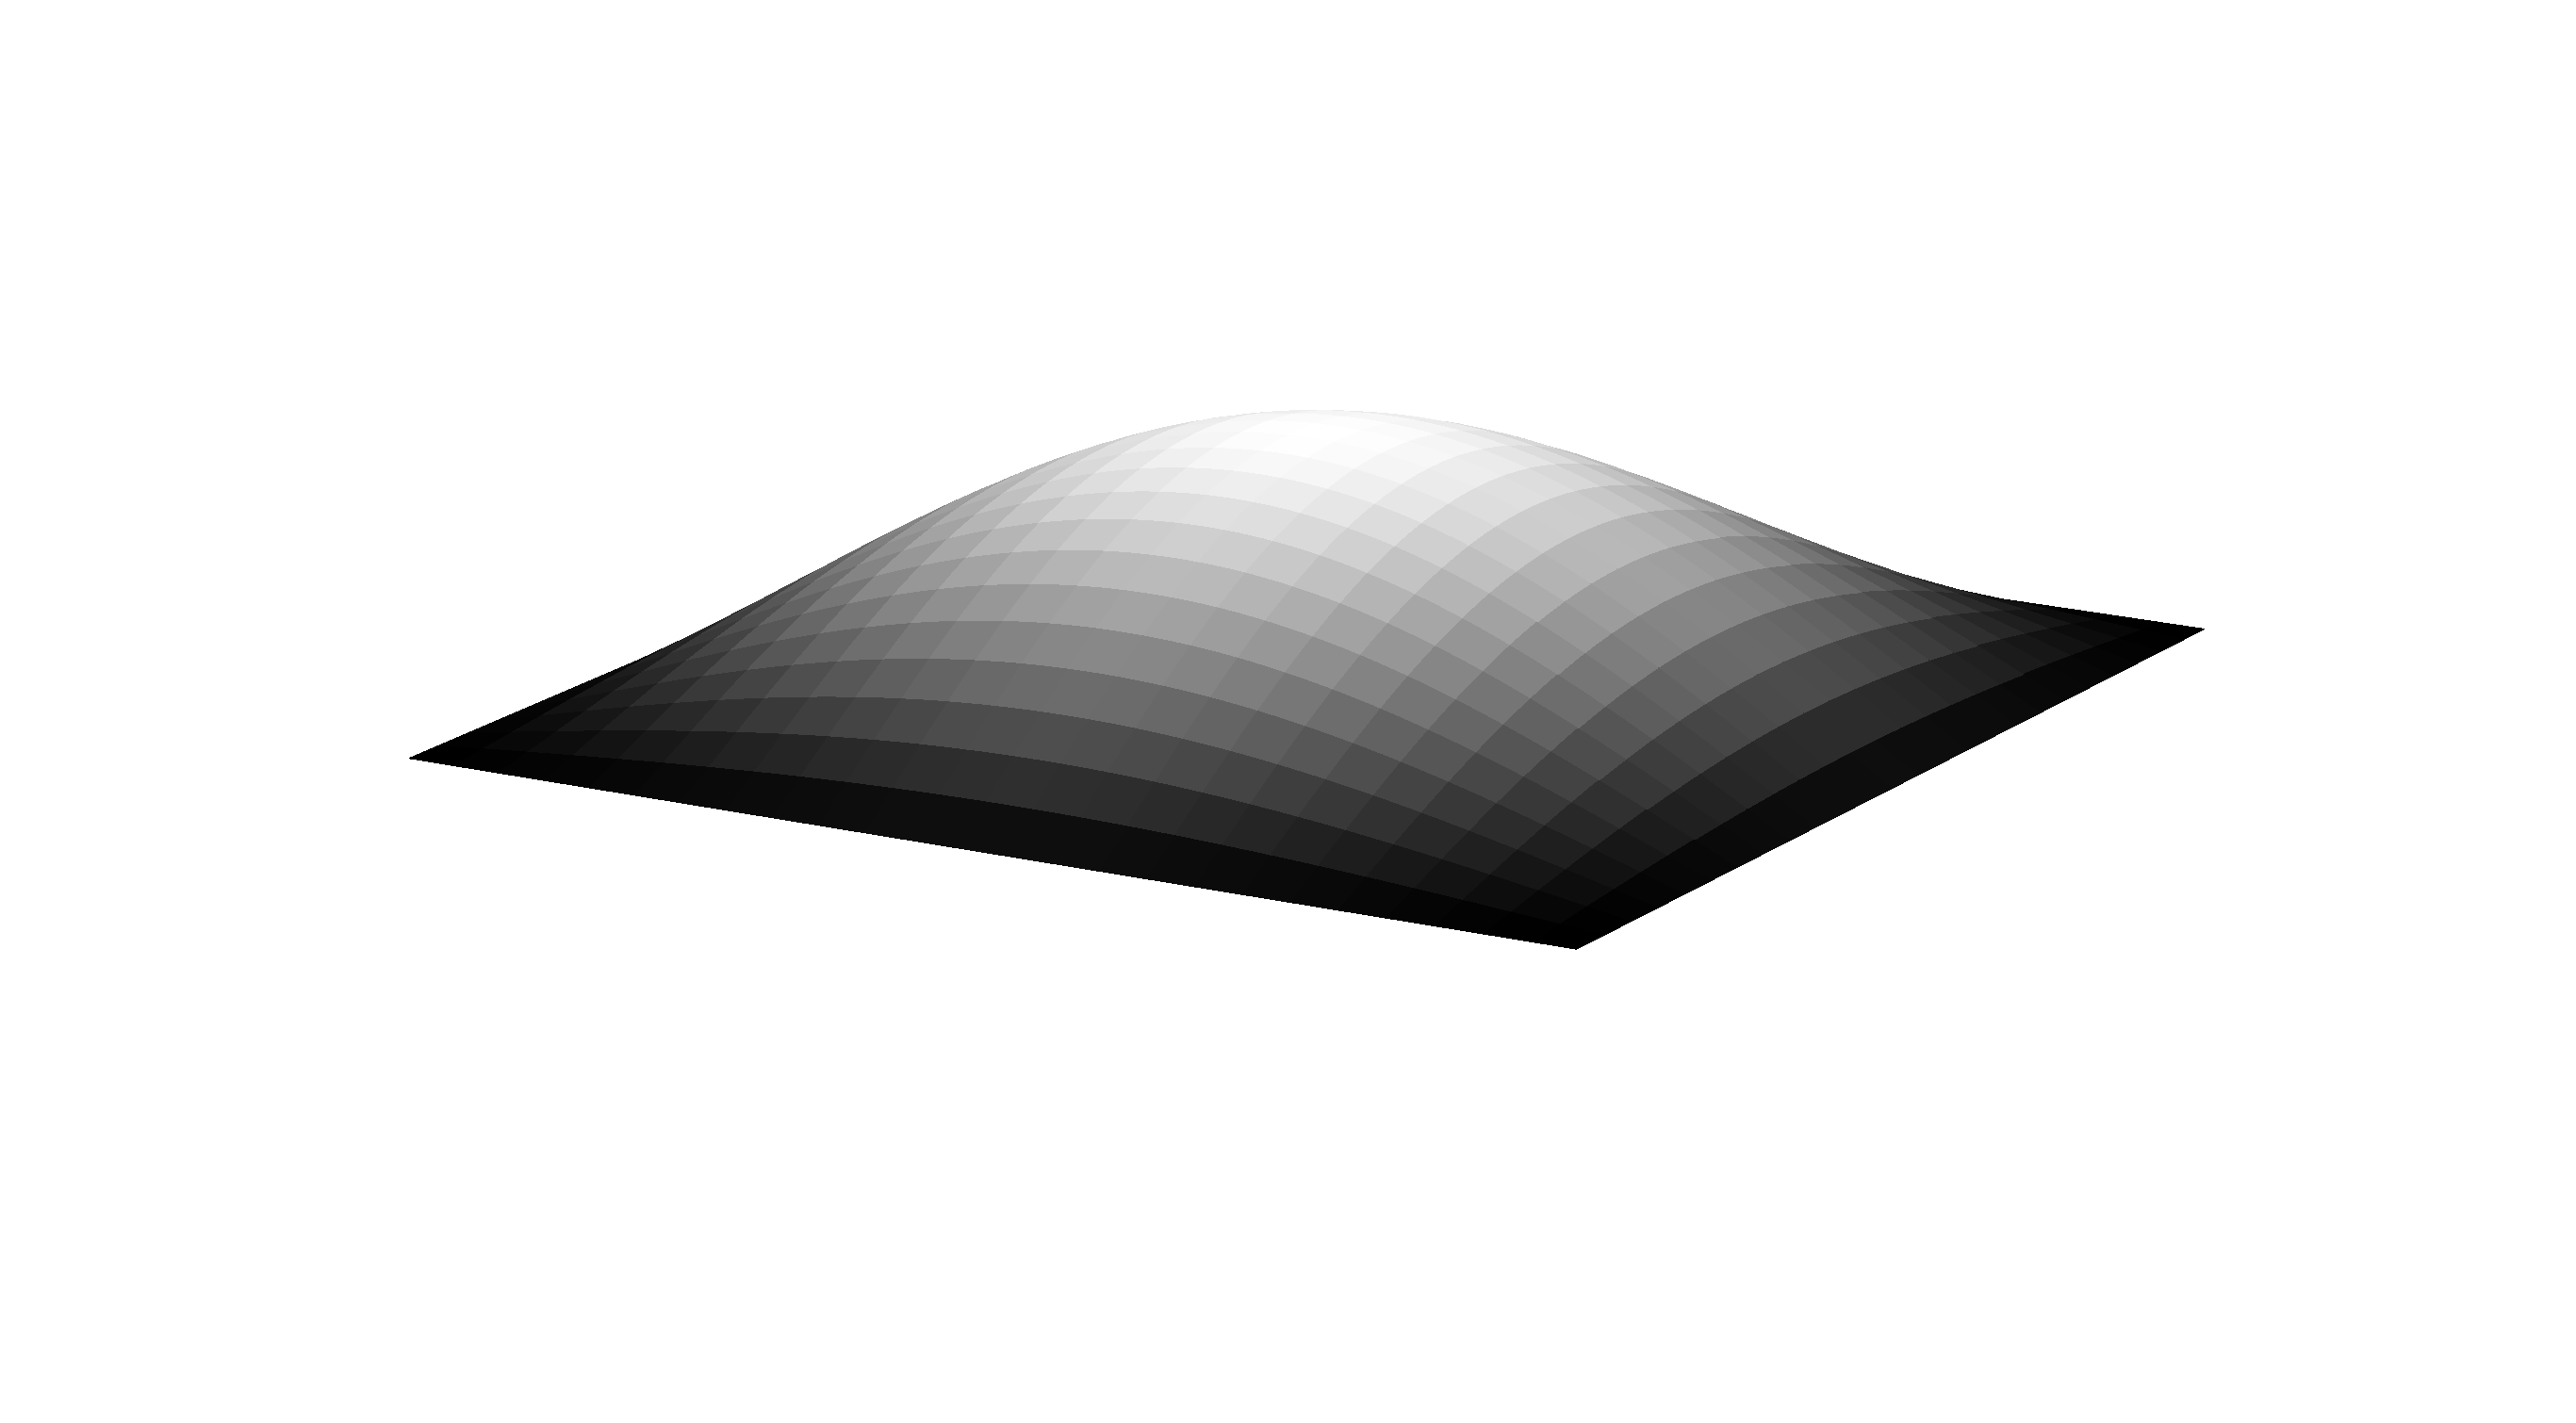
\includegraphics[width=\textwidth]{/modes/mode11.eps}
        \caption*{(1,1)}
    \end{subfigure}
    \hfil
    \begin{subfigure}[b]{0.49\textwidth}
        \centering
        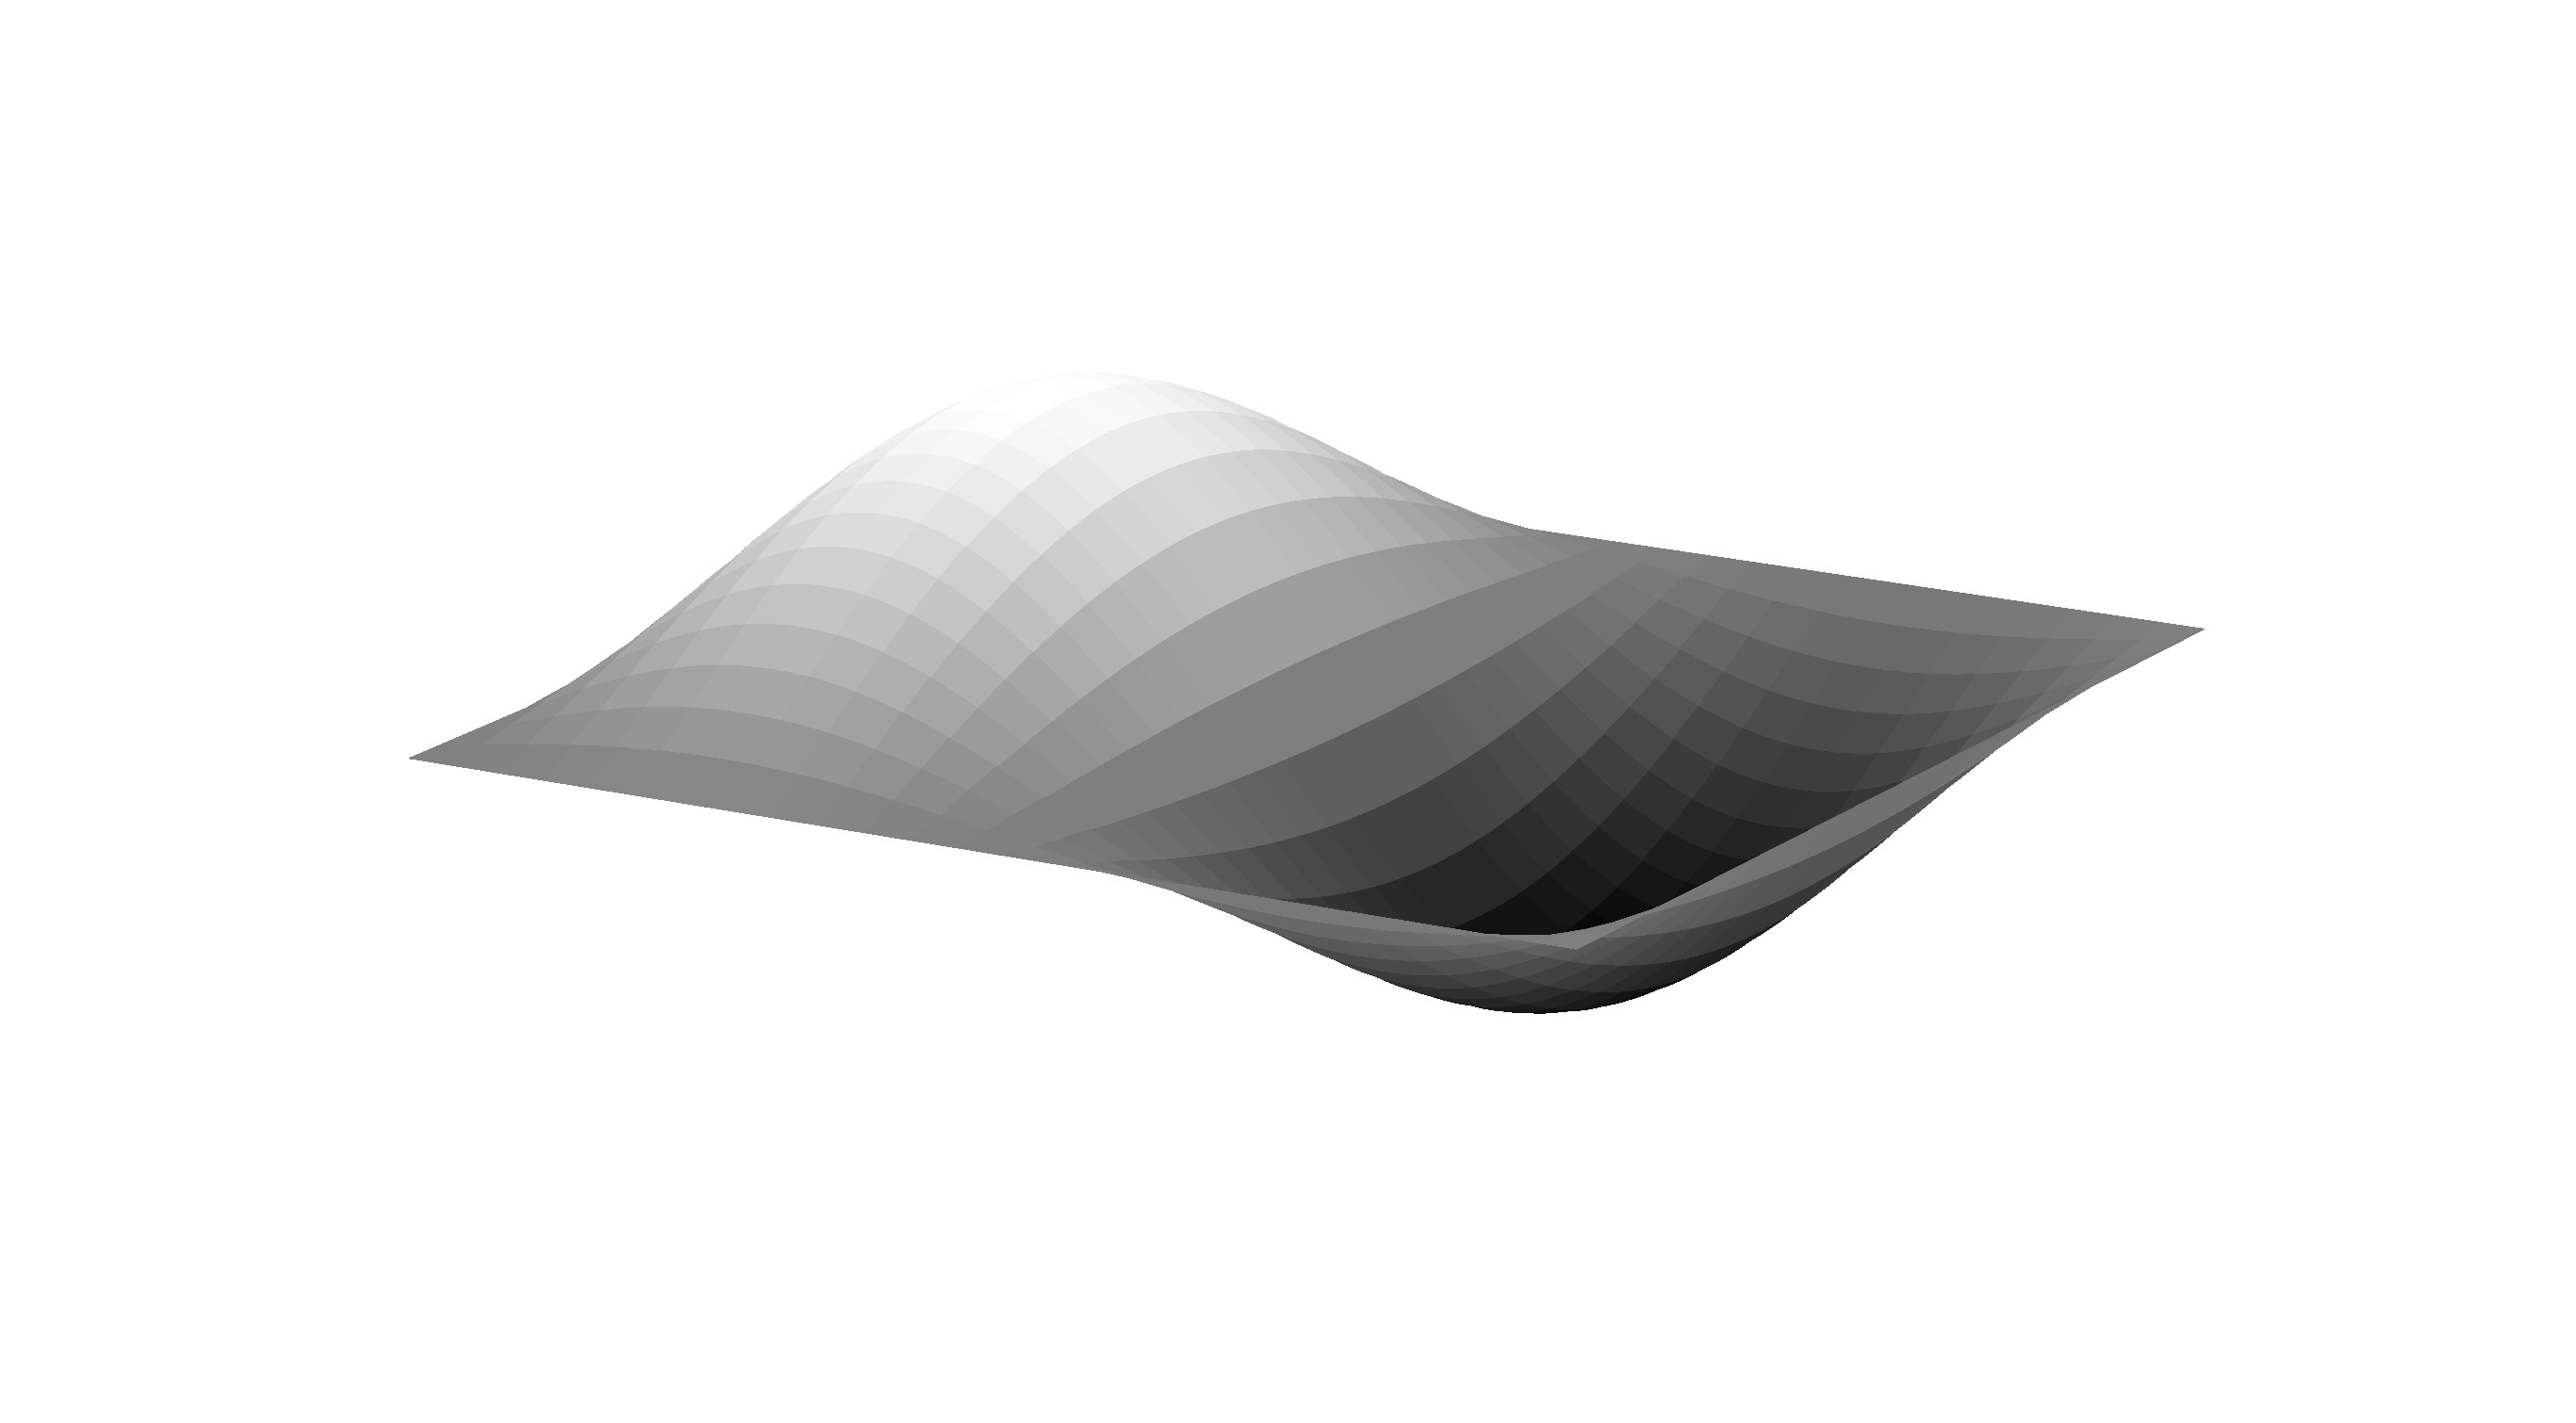
\includegraphics[width=\textwidth]{/modes/mode12.eps}
        \caption*{(1,2)}
    \end{subfigure}\\
    \begin{subfigure}[b]{0.49\textwidth}
        \centering
        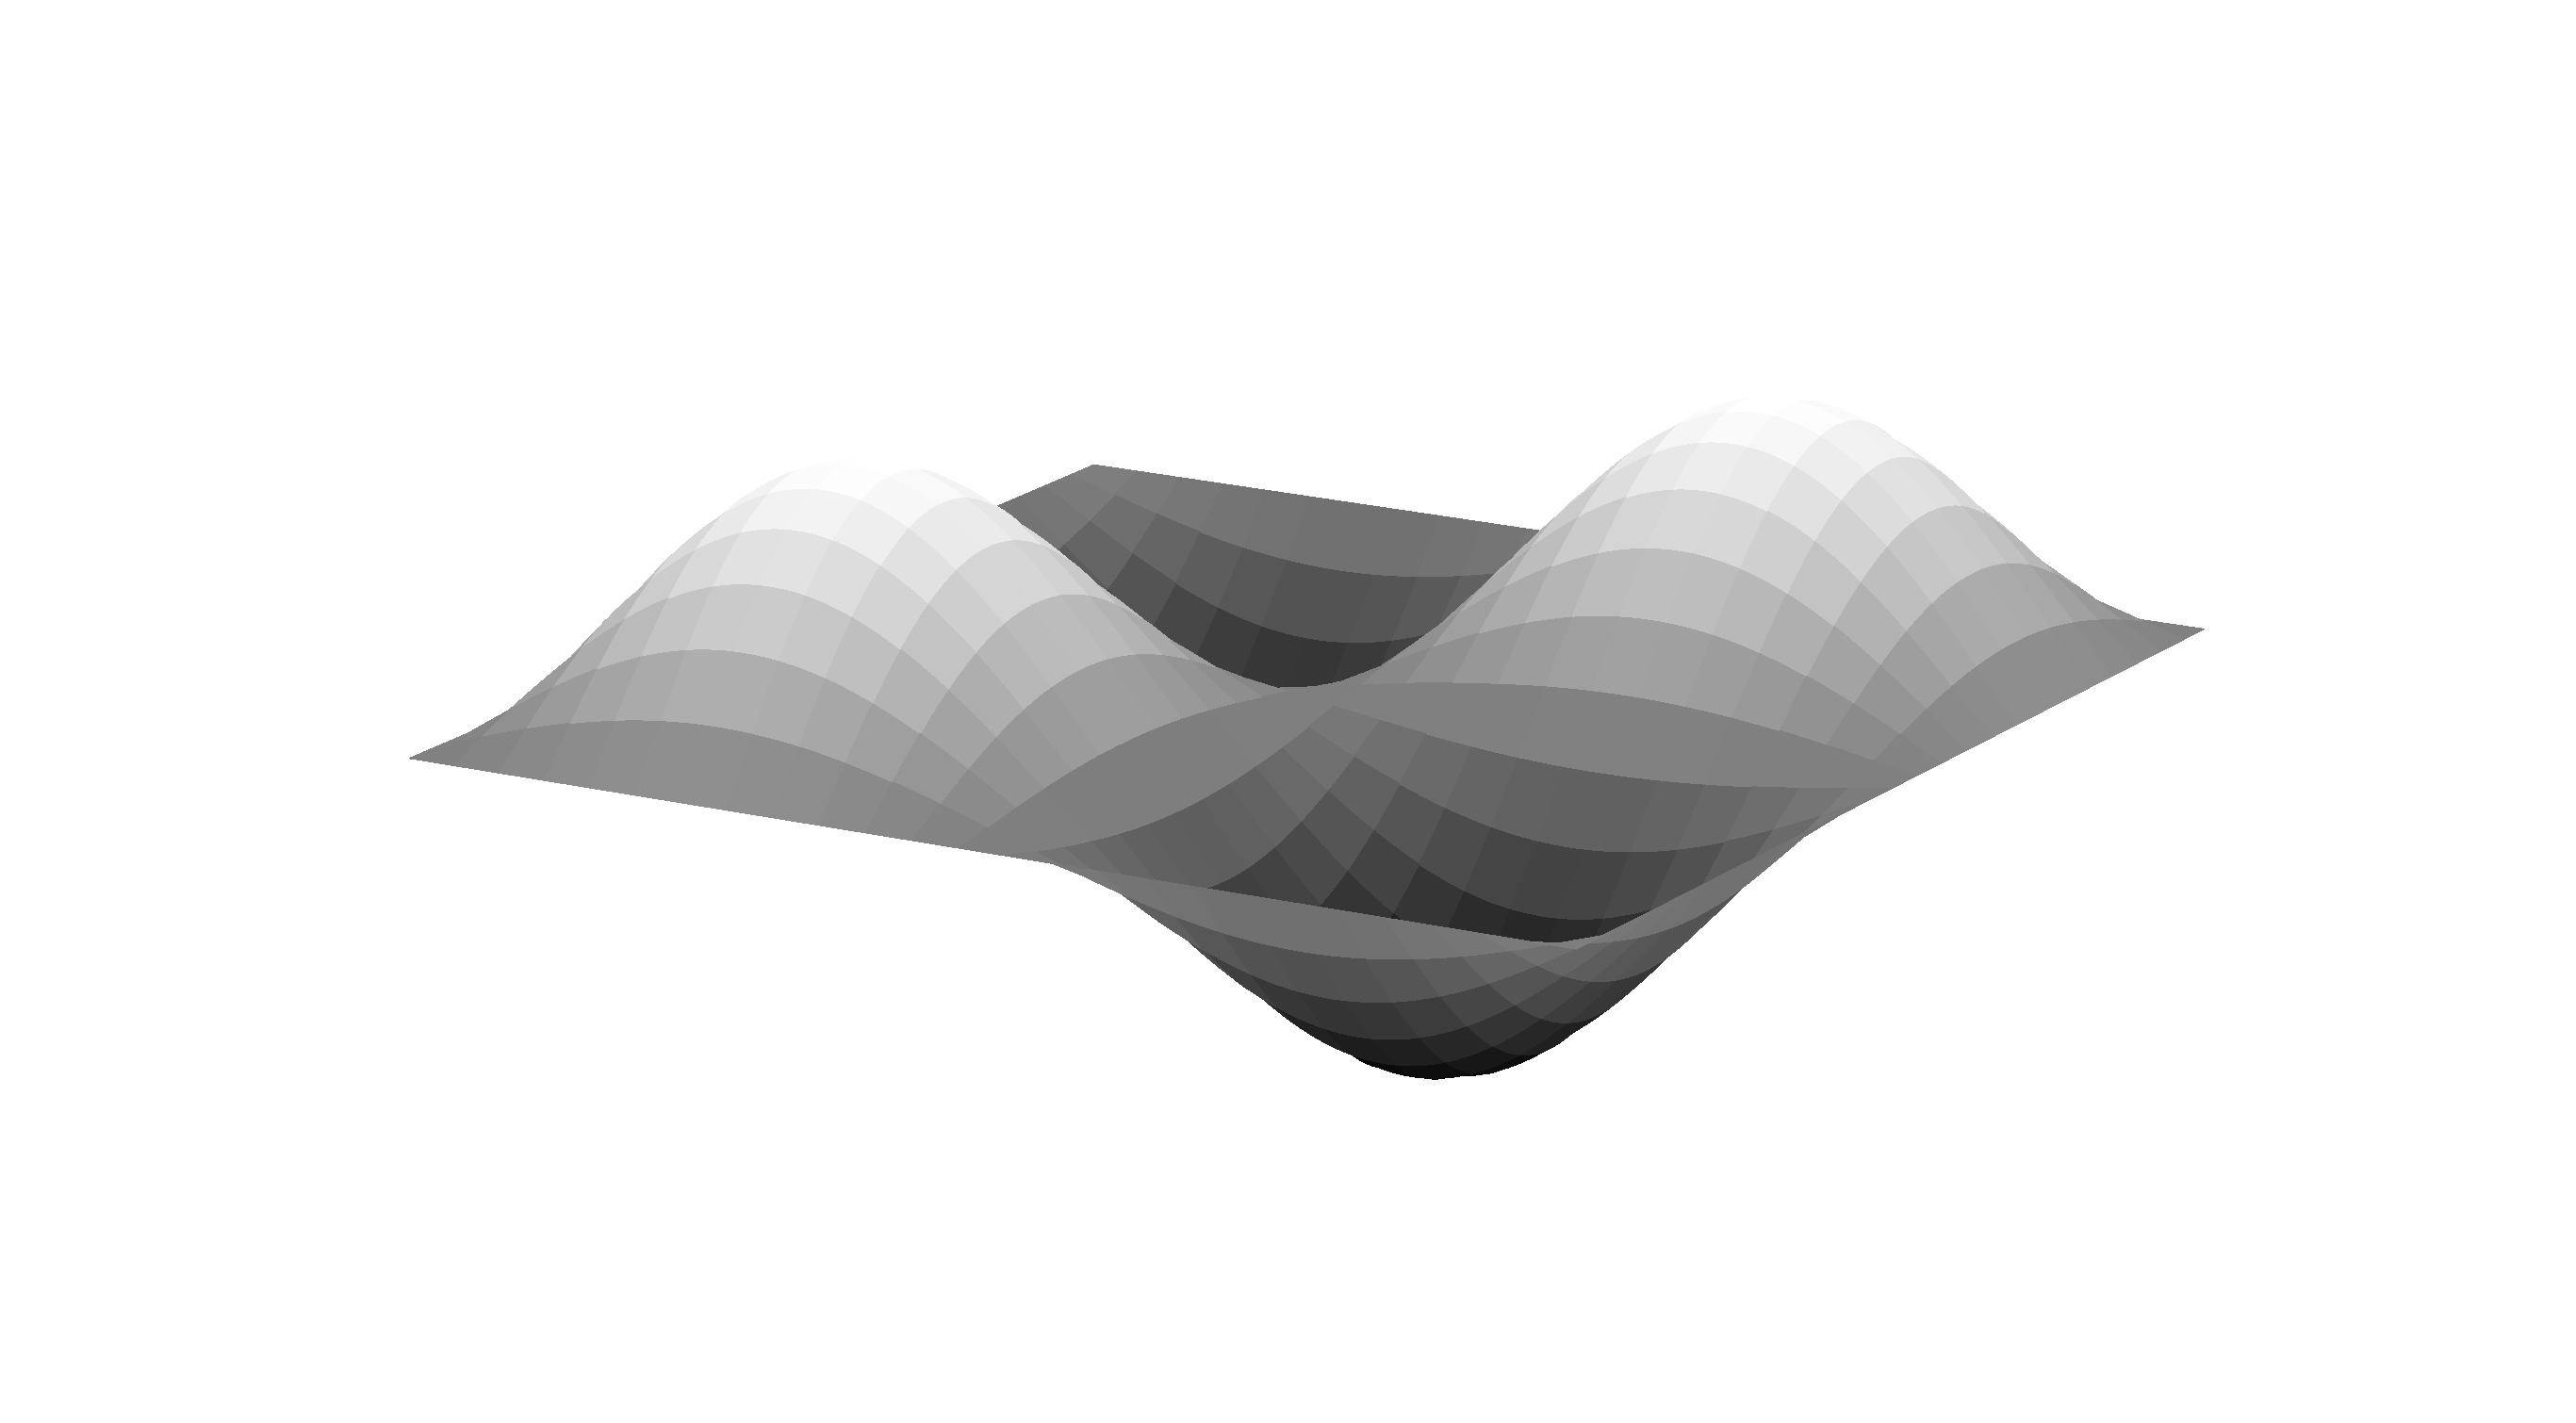
\includegraphics[width=\textwidth]{/modes/mode22.eps}
        \caption*{(2,2)}
    \end{subfigure}
    \hfil
    \begin{subfigure}[b]{0.49\textwidth}
        \centering
        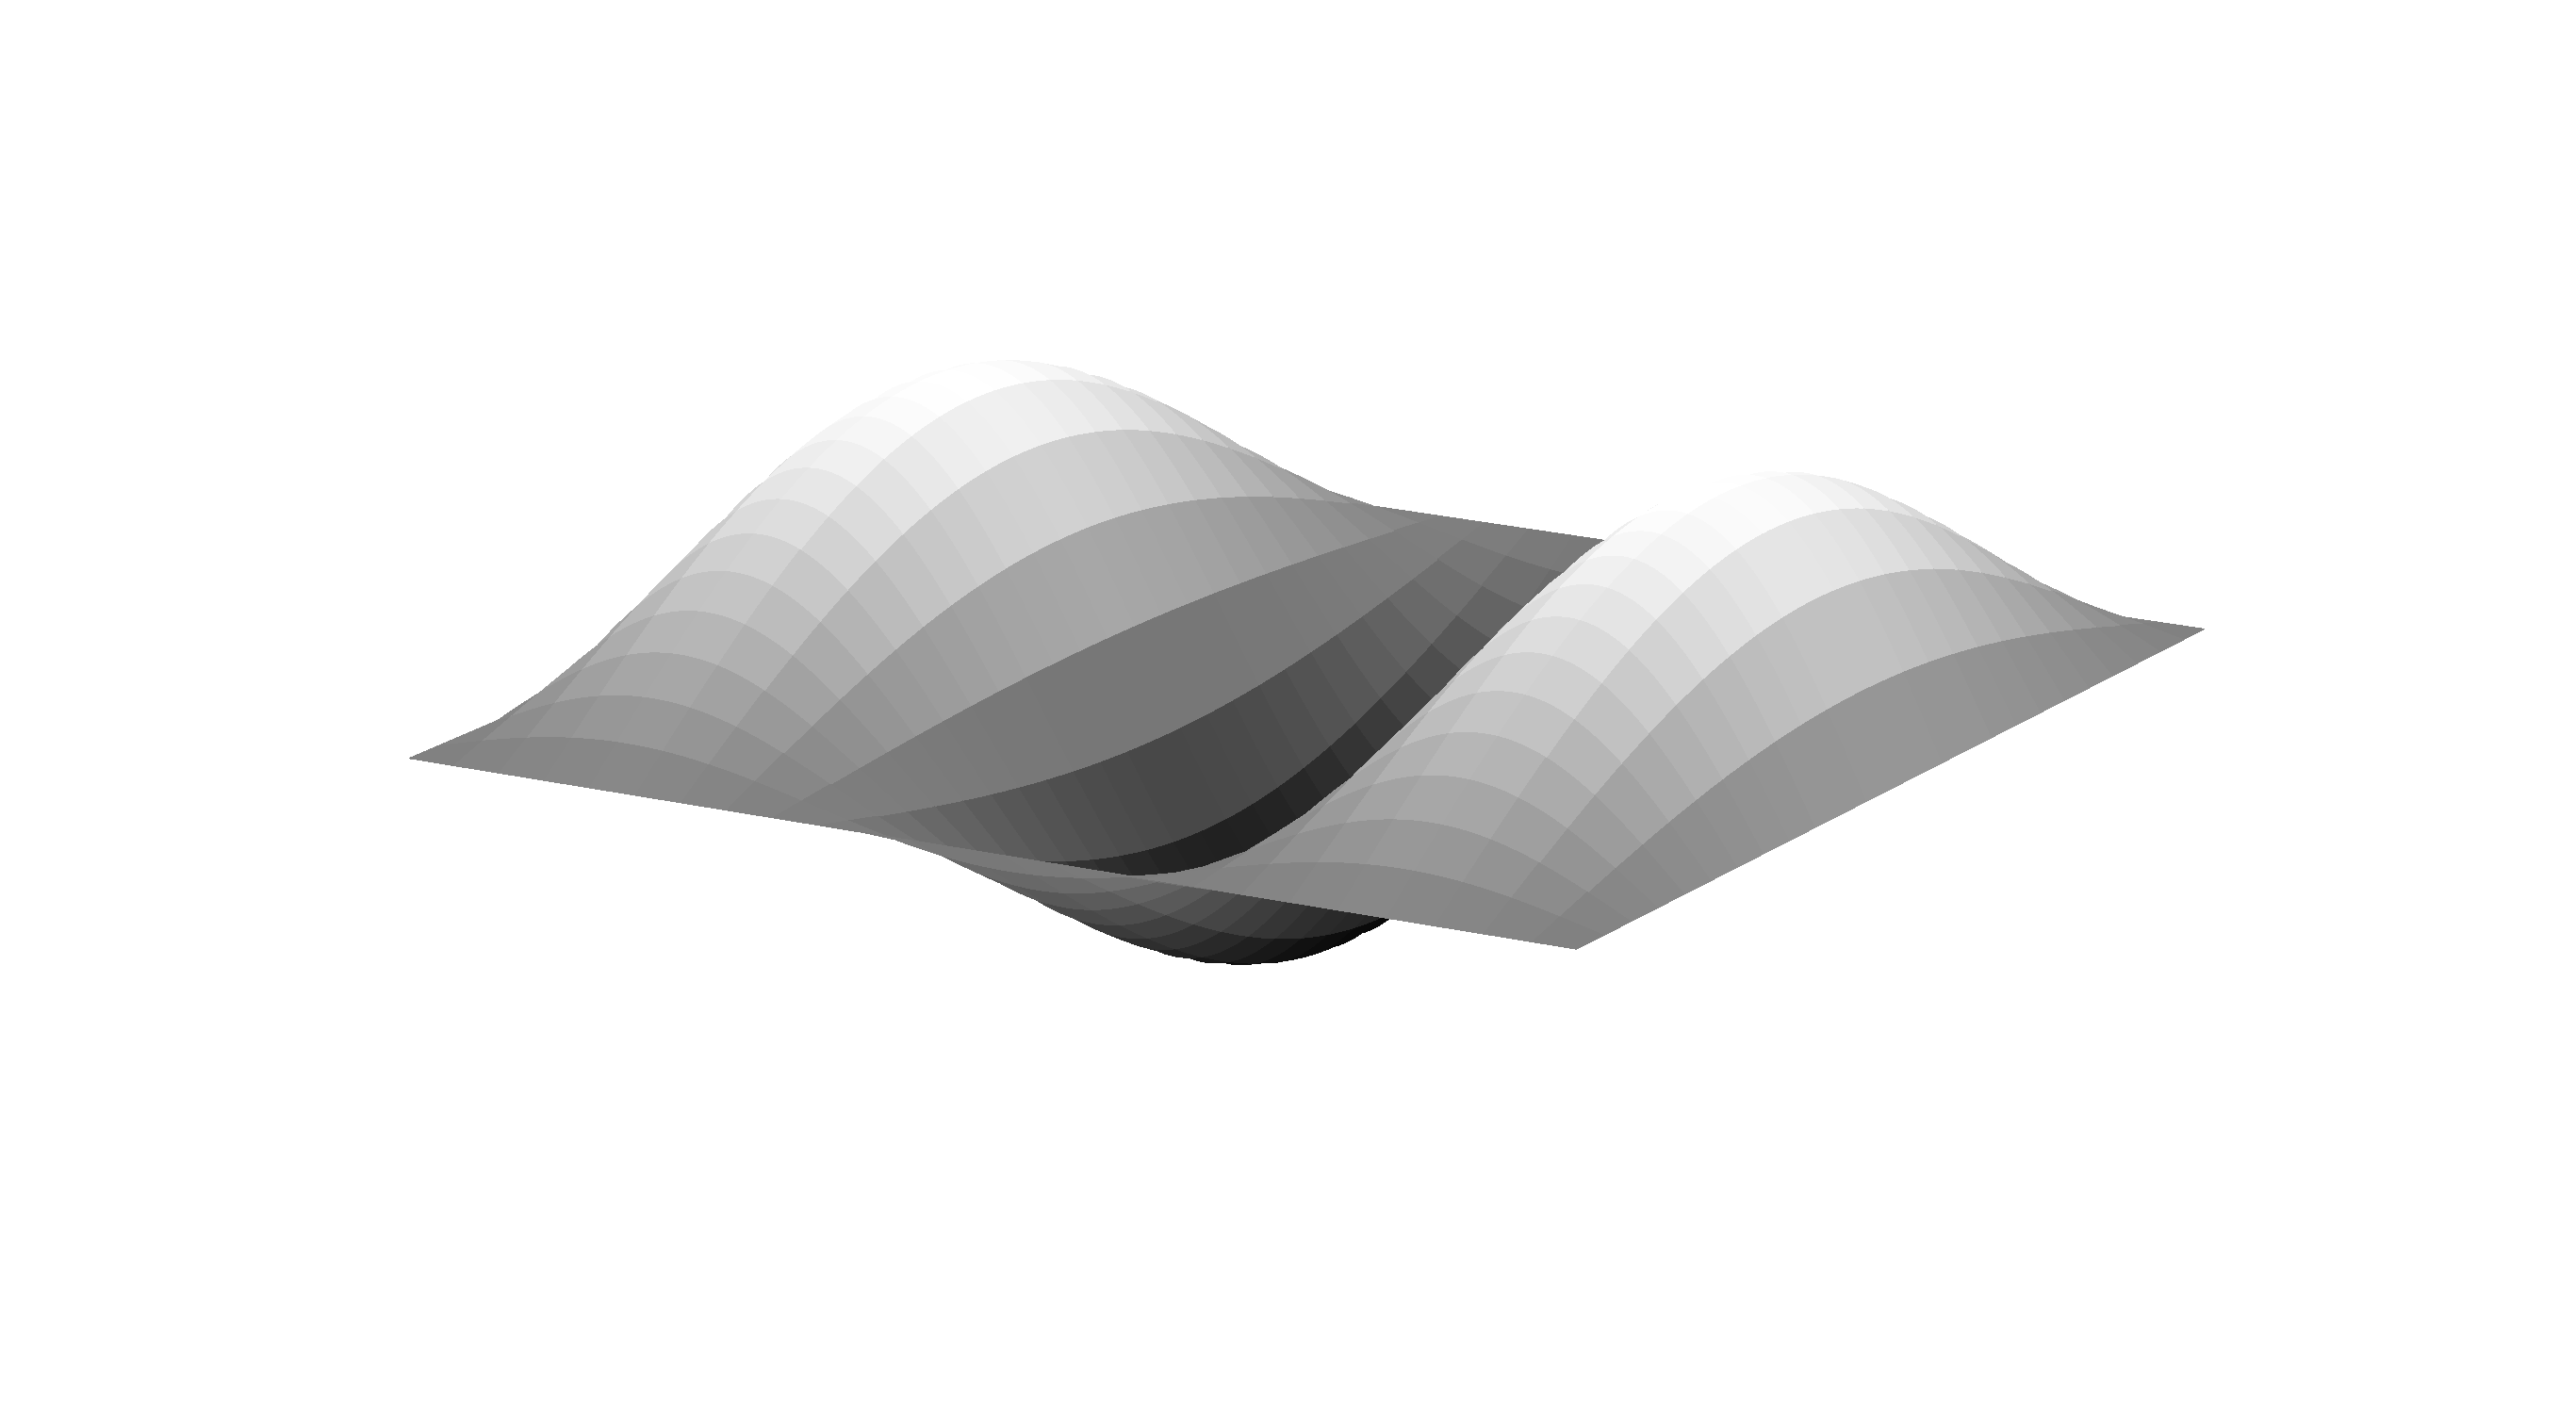
\includegraphics[width=\textwidth]{/modes/mode13.eps}
        \caption*{(1,3)}
    \end{subfigure}\\
        \begin{subfigure}[b]{0.49\textwidth}
        \centering
        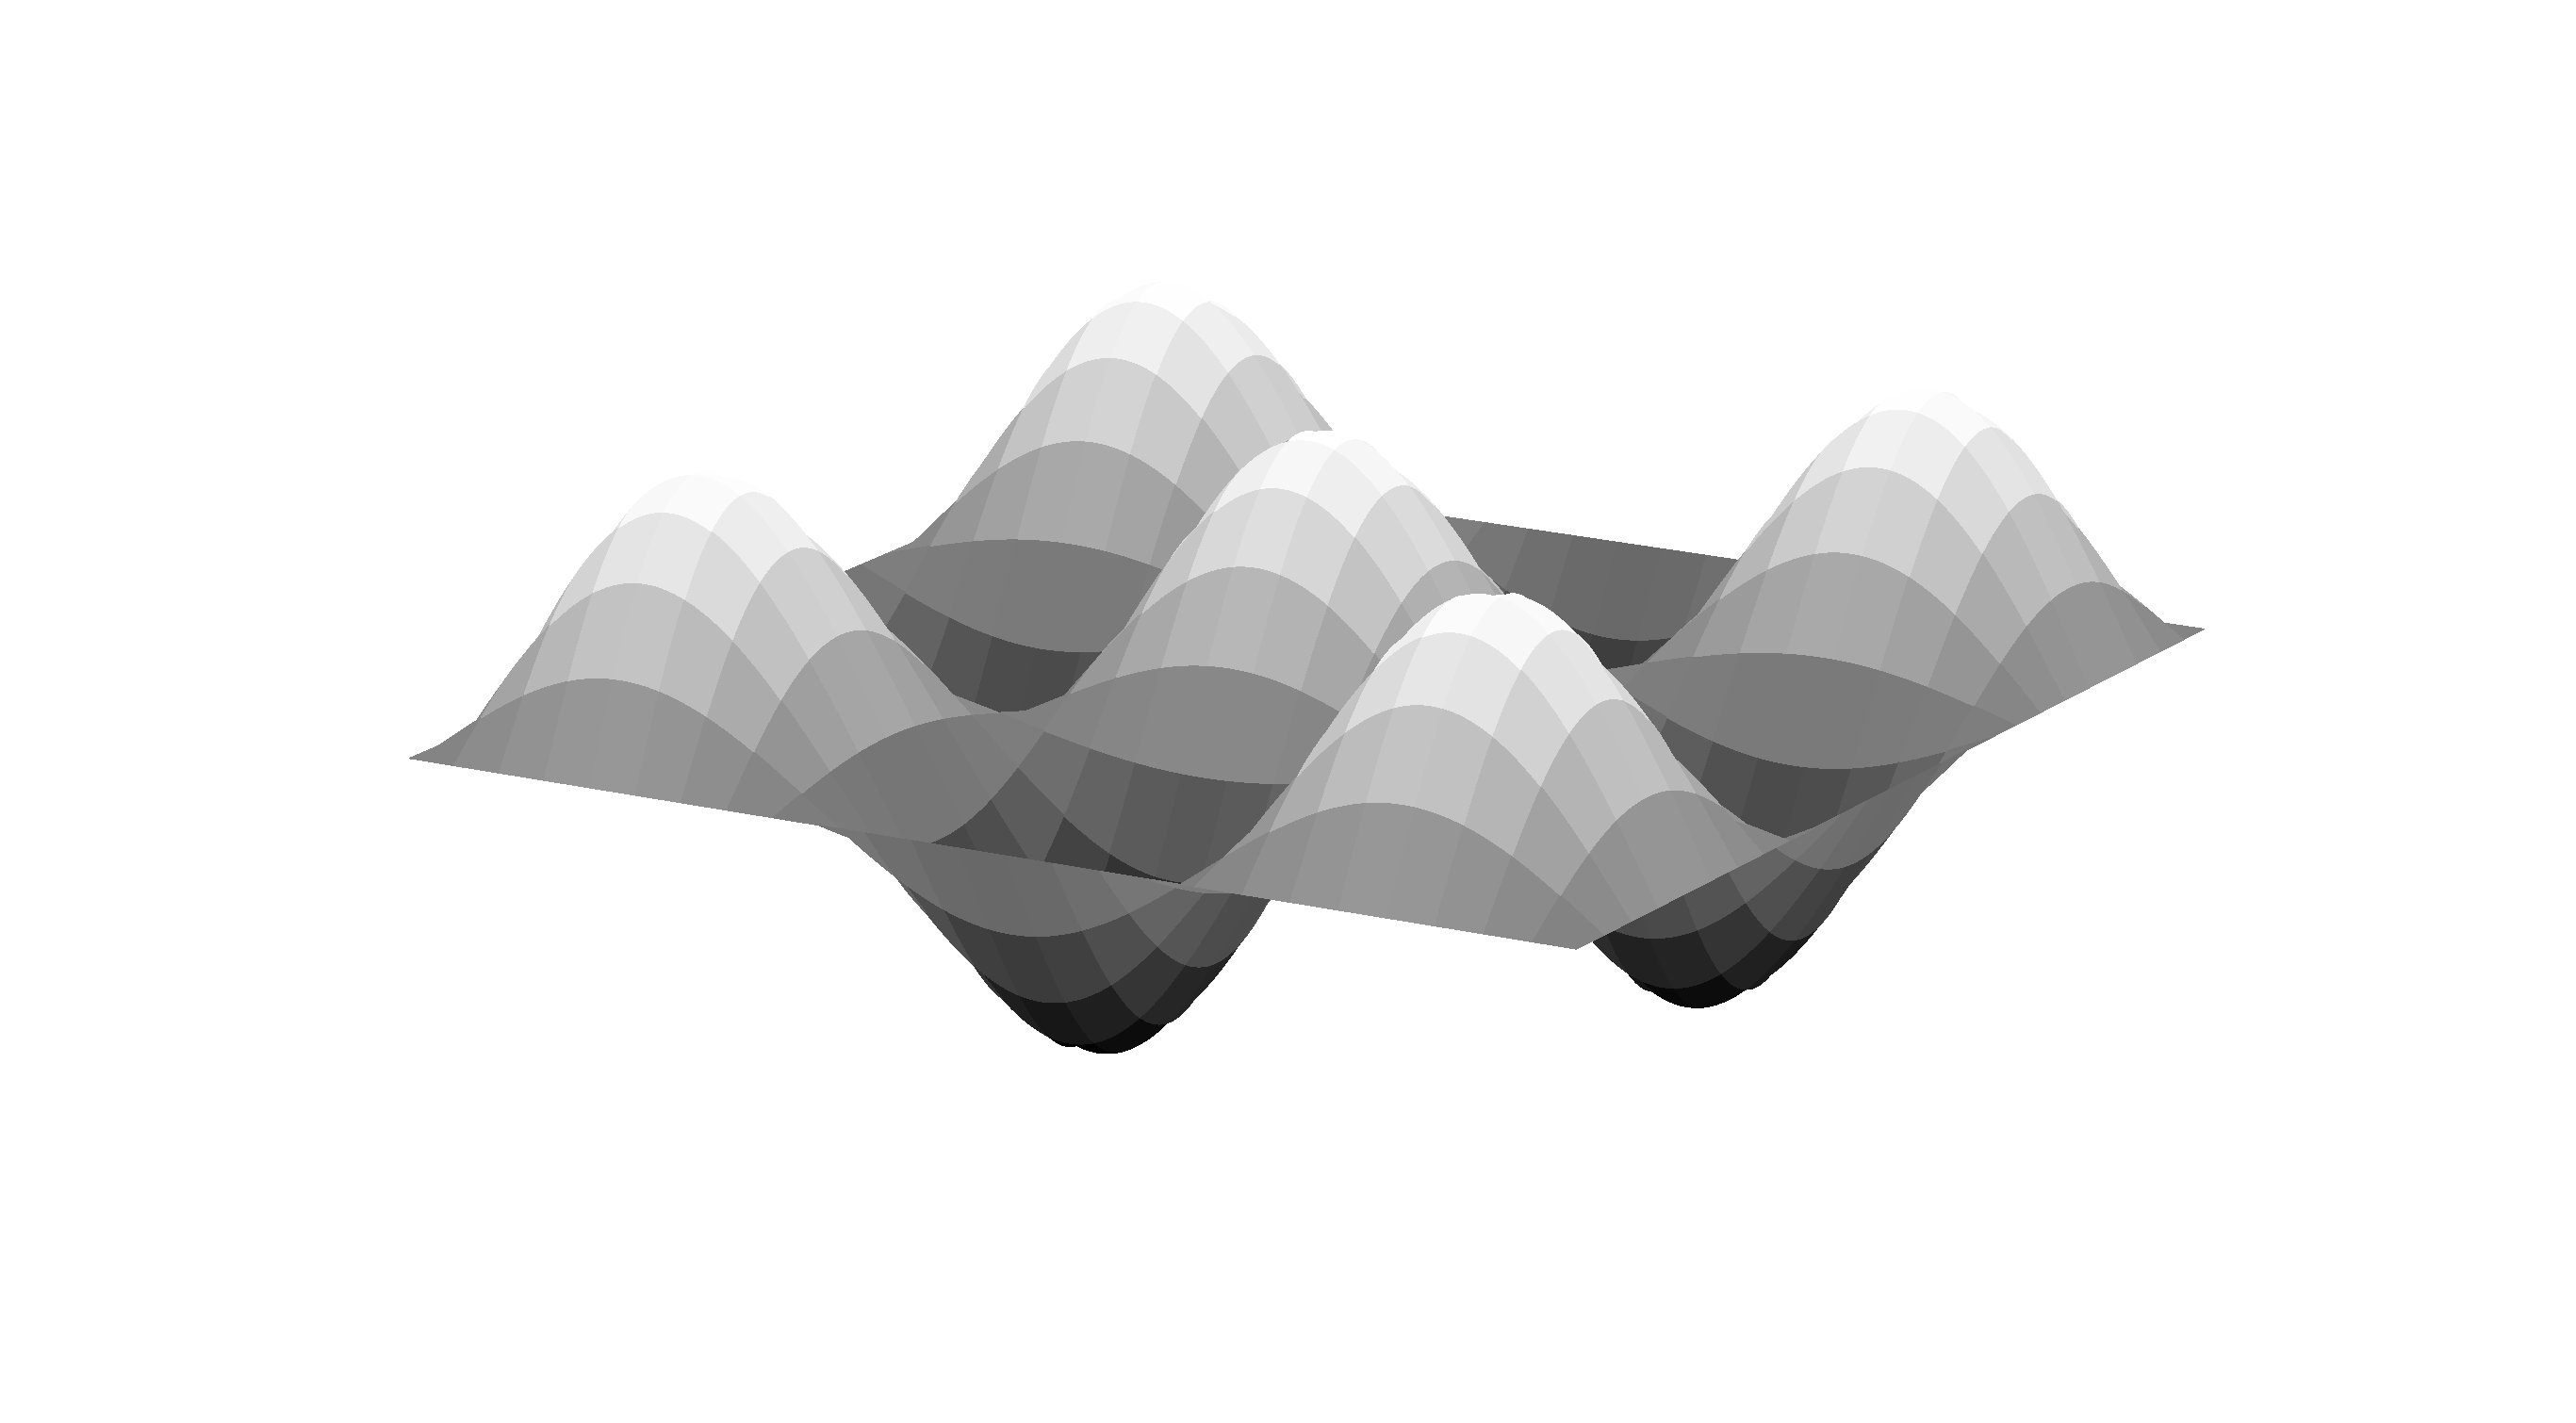
\includegraphics[width=\textwidth]{/modes/mode33.eps}
        \caption*{(3,3)}
    \end{subfigure}
    \hfil
    \begin{subfigure}[b]{0.49\textwidth}
        \centering
        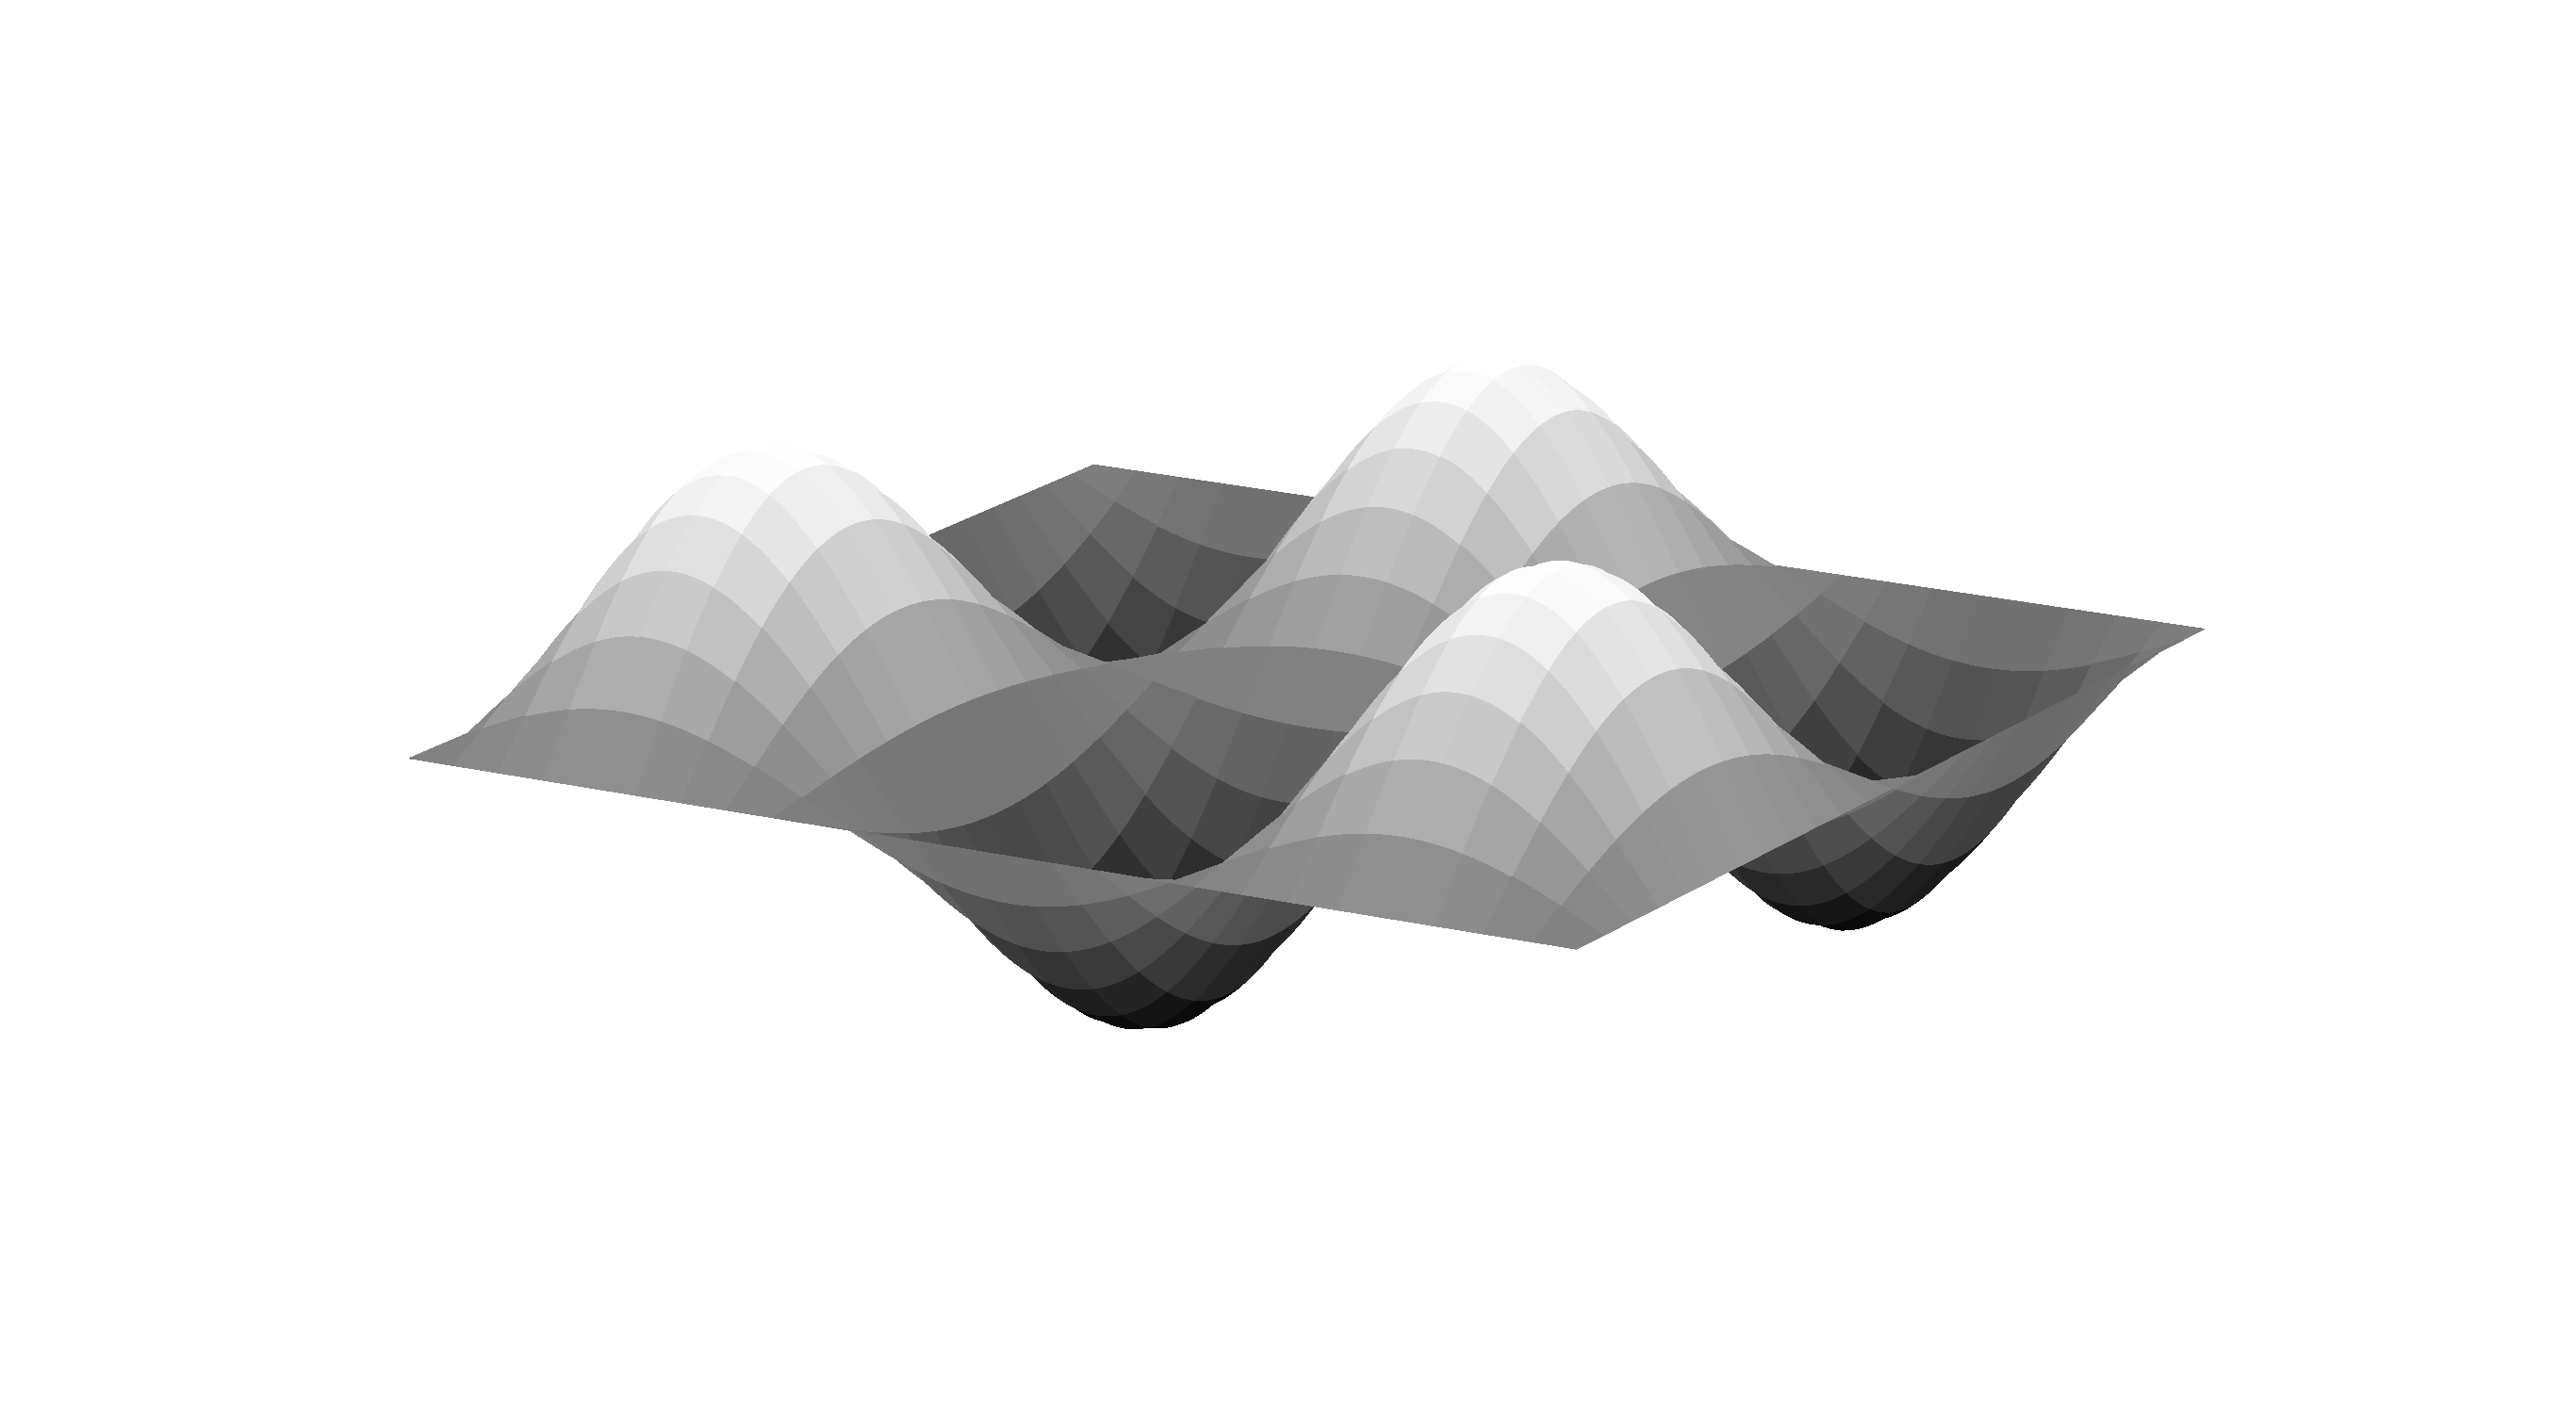
\includegraphics[width=\textwidth]{/modes/mode23.eps}
        \caption*{(2,3)}
    \end{subfigure}
\caption{Examples of vibrational mode shapes $(m, n)$ for the square membrane with all amplitudes normalized to unity.}
\label{fig:modeshape}
\end{figure}

Later we will mostly refer to a specific mechanical angular eigenfrequencies as $\Omega_m$, but the previous definition $\Omega_{m,n}$ is still valid.